%%%%%%%%%%%%%%%%%%%%%%%%%%%%%%%%%%%%%%%%%%%%%%%%%%%%%%%%%%%%%%%%%%%%%%%%%%%%
% Author: Manuel López-Ibáñez <manuel.lopez-ibanez@ulb.ac.be>
%
% License: Copyright  Manuel López-Ibáñez
%          CC-BY-3.0 http://creativecommons.org/licenses/by/3.0/
%
%%%%%%%%%%%%%%%%%%%%%%%%%%%%%%%%%%%%%%%%%%%%%%%%%%%%%%%%%%%%%%%%%%%%%%%%%%%
\documentclass[xcolor={x11names},12pt,plain,usepdftitle=false]{beamer}
\setbeamertemplate{navigation symbols}{} 
\usepackage{tikz}
\usetikzlibrary{arrows,trees,shapes}%,positioning}
\usepackage{amssymb,amsmath}
\hypersetup{pdfauthor={Manuel Lopez-Ibanez},
            pdftitle={The Racing Approach},%
            pdfsubject={Copyright  Manuel López-Ibáñez CC-BY-3.0},
            pdfkeywords={Tuning, Race}}%

% Example of overriding labels.          
\newcommand{\raceConfigurations}{$\Theta$}

% This test is based on original code from Mauro Birattari.
\begin{document}
\begin{frame}
  \begin{columns}
    \begin{column}{.35\textwidth}
      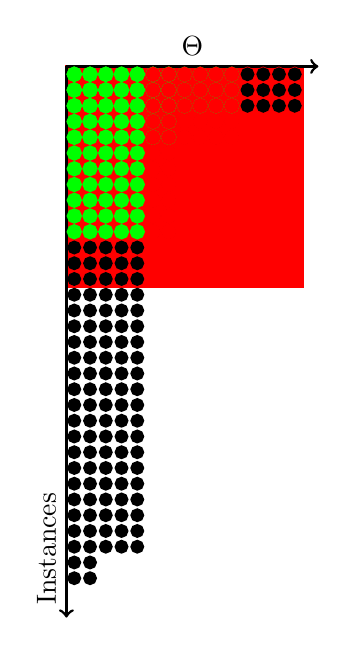
\begin{tikzpicture}[scale=0.2]
        %%%%%%%%%%%%%%%%%%%%%%%%%%%%%%%%%%%%%%%%%%%%%%%%%%%%%%%%%%%%%%%%%%%%%%%%%%%%
% Author: Manuel López-Ibáñez <manuel.lopez-ibanez@ulb.ac.be>
%
% License: Copyright  Manuel López-Ibáñez
%          CC-BY-3.0 http://creativecommons.org/licenses/by/3.0/
%%%%%%%%%%%%%%%%%%%%%%%%%%%%%%%%%%%%%%%%%%%%%%%%%%%%%%%%%%%%%%%%%%%%%%%%%%

\providecommand{\raceConfigurations}{$\Theta$}

\tikzstyle{hidden} = [white,color=white];
\tikzstyle{unselected} = [black,color=black];
\tikzstyle{selected} = [green,color=green, line width=1.5pt];
\tikzstyle{discarded} = [red,color=red, line width=1.5pt];

\tikzstyle{every node}=[font=\normalsize];
\tikzstyle{every path} = [line width=1pt];
\tikzstyle{arrow1} = [black,color=black];
\tikzstyle{arrow2} = [black,color=black];

%%% Local Variables: 
%%% mode: latex
%%% TeX-master: t
%%% End: 

        %%%-*- mode: latex; TeX-master: "race-test"-*-%
%%%%%%%%%%%%%%%%%%%%%%%%%%%%%%%%%%%%%%%%%%%%%%%%%%%%%%%%%%%%%%%%%%%%%%%%%%
% Author: Manuel López-Ibáñez <manuel.lopez-ibanez@ulb.ac.be>
%
% License: Copyright  Manuel López-Ibáñez
%          CC-BY-3.0 http://creativecommons.org/licenses/by/3.0/
%
%%%%%%%%%%%%%%%%%%%%%%%%%%%%%%%%%%%%%%%%%%%%%%%%%%%%%%%%%%%%%%%%%%%%%%%%%%%
%% FIXME: 
%%
%% * Make it more compact. Draw the points once, and then use
%% \tikstyle to hide/show/color them.
%% * Fix overfull \hbox (it is caused by \raceConfigurations).
%% * Make it more configurable:
%%    - Calculate \ystart \yend w.r.t. \rows (how to do computations in tikz?)
%%    - Define variable for circle size.
%%    - Define variable for transitions.
%%    - Define commands for labels.

%\draw[style=help lines] (0,0) grid (1,45);

\def\rows{35}
\def\ystart{34.5}
\def\yend{32.5}

\onslide*<.(17)->{
  \tikzstyle{unselected} = [selected]
}
\onslide*<.(18)>{
  \draw[fill=red,draw,red] (0,\rows) rectangle (15,21);
}

\onslide*<+>{
  \foreach \y in {0} {
    \foreach \x in {0,...,14}
    \filldraw[unselected] (0.5 + \x  , \ystart - \y) circle (0.35);
  }
}

\onslide*<+>{
\tikzstyle{arrow2} = [line width=1.5pt,red];
}
\onslide*<+>{
\tikzstyle{arrow1} = [line width=1.5pt,red];
}

\draw[arrow1,->]  (0,\rows) -- (0,0) node[very near end,above,rotate=90]{Instances};
\draw[arrow2,->]  (0,\rows) -- (16,\rows) node[midway,above]{\raceConfigurations};



\foreach \y in {0,...,2} {
  \foreach \x in {0,...,14}
  \filldraw[unselected] (0.5 + \x  , \ystart - \y) circle (0.35);
  \pause
}

\onslide*<+>{
  \foreach \y in {0,...,2} {
    \foreach \x in {0,...,10}
    \filldraw[selected] (0.5 + \x  , \ystart - \y) circle (0.35);
    \foreach \x in {11,...,14}
    \filldraw[discarded] (0.5 + \x  , \ystart - \y) circle (0.35);
  }
}

\onslide*<+->{
  \foreach \y in {0,...,2} {
    \foreach \x in {0,...,14}
    \filldraw[unselected] (0.5 + \x  , \ystart - \y) circle (0.35);
  }

  \foreach \y in {3} {
    \foreach \x in {0,...,10}
    \filldraw[unselected] (0.5 + \x  , \ystart - \y) circle (0.35);
  }
}

\onslide*<+->{
  \foreach \y in {4} {
    \foreach \x in {0,...,10}
    \filldraw[unselected] (0.5 + \x  , \ystart - \y) circle (0.35);
  }
}

\onslide*<+>{
  \foreach \y in {0,...,4} {
     \foreach \x in {0,...,6}
     \filldraw[selected] (0.5 + \x, \ystart - \y) circle (0.35);
     \foreach \x in {7,...,10}
     \filldraw[discarded] (0.5 + \x, \ystart - \y) circle (0.35);
   }
}

\onslide*<+->{
  \foreach \y in {5} {
    \foreach \x in {0,...,6}
    \filldraw[unselected] (0.5 + \x  , \ystart - \y) circle (0.35);
  }
}

\onslide*<+->{
  \foreach \y in {6,...,10} {
    \foreach \x in {0,...,6}
    \filldraw[unselected] (0.5 + \x  , \ystart - \y) circle (0.35);
  }
}

\onslide*<+>{
  \foreach \y in {0,...,10} {
    \foreach \x in {0,...,4}
    \filldraw[selected] (0.5 + \x  , \ystart - \y) circle (0.35);
    \foreach \x in {5,...,6}
    \filldraw[discarded] (0.5 + \x  , \ystart - \y) circle (0.35);
  }
}

\onslide*<+->{
  \foreach \y in {11,...,20} {
    \foreach \x in {0,...,4}
    \filldraw[unselected] (0.5 + \x  , \ystart - \y) circle (0.35);
  }
}

\onslide*<+->{
  \foreach \y in {21,...,30} {
    \foreach \x in {0,...,4}
    \filldraw[unselected] (0.5 + \x  , \ystart - \y) circle (0.35);
  }
}

\onslide*<+->{
  \foreach \y in {31,...,\yend} {
    \foreach \x in {0,...,1}
    \filldraw[unselected] (0.5 + \x  , \ystart - \y) circle (0.35);
  }
}




      \end{tikzpicture}
    \end{column}
    \begin{column}{.65\textwidth}
      % Following Maron and Moore (1994):
      \begin{itemize}
      \item<2-| alert@2> start with a set of initial candidates
	\item<3-| alert@3> consider a \emph{stream} of instances
	\item<4-| alert@4-6,9,12> sequentially evaluate candidates 
	\item<7-> \alert<7,10,13>{discard inferior candidates}\\
	  \visible<7->{{\footnotesize as sufficient evidence is gathered against them}}
	\item<visible@16-> \alert<16>{\dots repeat until a winner is selected}\\
	  \visible<16->{{\footnotesize or until computation time expires}}  
        \end{itemize}
        \bigskip
      \end{column}
    \end{columns}
\end{frame}
\end{document}


%%% Local Variables: 
%%% mode: latex
%%% TeX-master: t
%%% End: 
